El Nivel Regulatorio constituye el sistema de control en tiempo real del robot. Su responsabilidad principal es la gestión directa de actuadores (motores paso a paso, servomotores, actuador de agarre) y sensores (finales de carrera), ejecutando comandos de movimiento recibidos desde el nivel supervisor.

El firmware se estructura en tres capas jerárquicas que separan las responsabilidades según el nivel de abstracción (Figura \ref{fig:arquitectura_regulatorio}):

\textbf{Capa de Controladores de Hardware (Drivers)}: Interactúa directamente con los periféricos del microcontrolador mediante registros y temporizadores. El controlador de motores paso a paso genera pulsos mediante Timer1 configurado en modo CTC (Clear Timer on Compare Match), alternando el estado del pin STEP en cada interrupción. Los controladores de servomotores utilizan señales PWM generadas por hardware mediante Timer4 y Timer5 con frecuencia de 50Hz. El controlador del actuador de agarre maneja el motor paso a paso 28BYJ-48 mediante secuencia de pasos programada. El controlador de comunicación serial implementa transmisión y recepción mediante interrupciones USART con buffer circular de 256 bytes.

\textbf{Capa de Control de Movimiento}: Implementa la generación de trayectorias mediante perfiles de velocidad. El módulo de perfiles trapezoidales (motion\_profile) calcula la velocidad instantánea en cada paso del movimiento aplicando aceleraciones constantes. El gestor de límites monitorea los finales de carrera mediante interrupciones externas, deteniendo los ejes al detectar activación. El coordinador de movimientos sincroniza los ejes horizontal y vertical mediante escalamiento proporcional de velocidades, garantizando trayectorias rectilíneas en el plano XY.

\textbf{Capa de Aplicación}: Proporciona la interfaz de alto nivel para comandos del sistema supervisor. El módulo de interpretación de comandos (command\_parser) analiza las instrucciones recibidas por UART utilizando una máquina de estados que detecta delimitadores y extrae parámetros. El protocolo de comunicación define mensajes ASCII con formato estructurado y códigos de respuesta. El módulo de configuración (system\_config.h) centraliza parámetros del sistema: conversiones mecánicas (pasos por milímetro), velocidades máximas permitidas, aceleraciones, y límites angulares de servomotores.

\begin{figure}[H]
    \centering
    % TODO: Insertar diagrama de capas del firmware regulatorio
    % Mostrar: Aplicación → Control → Drivers → Hardware
    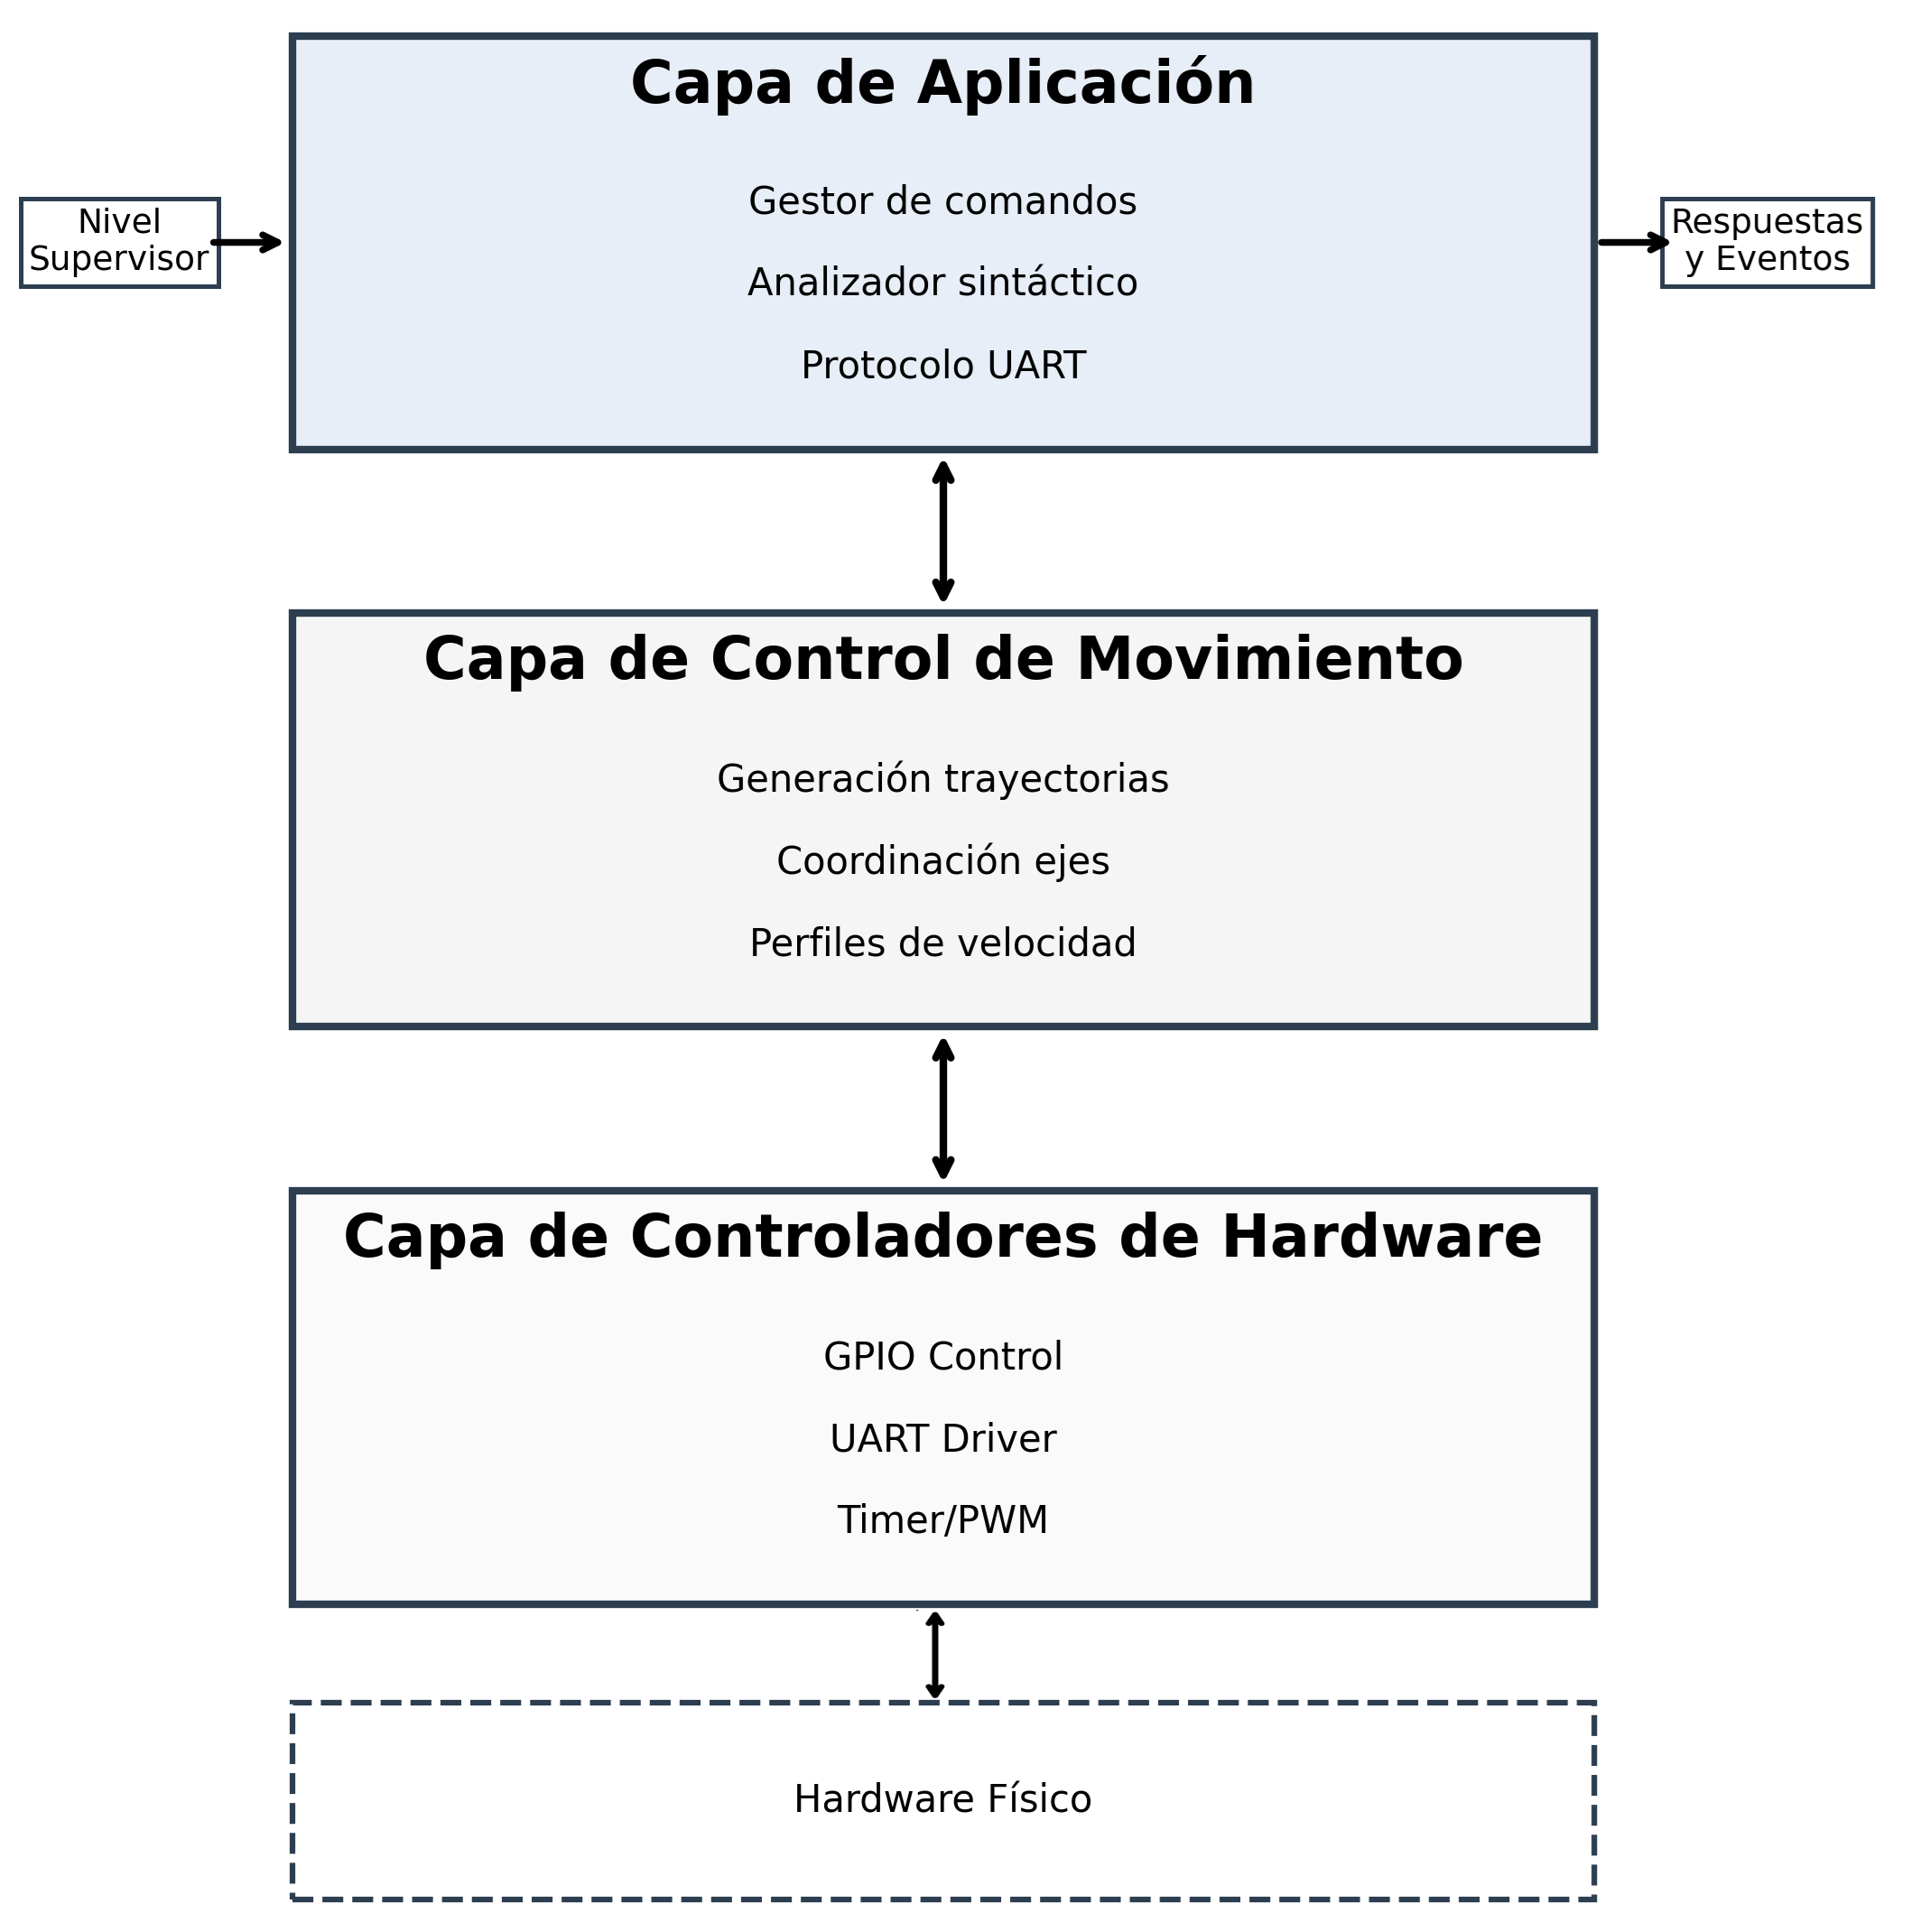
\includegraphics[width=0.6\textwidth]{imagenes/arquitectura_regulatorio_capas.png}
    \caption{Arquitectura en capas del firmware del Nivel Regulatorio}
    \label{fig:arquitectura_regulatorio}
\end{figure}

El flujo de procesamiento de un comando sigue la secuencia: recepción del mensaje por UART → análisis sintáctico en command\_parser → configuración de motion\_profile → generación de interrupciones en Timer1 → emisión de pulsos STEP hacia los drivers → notificación de finalización al supervisor. Esta arquitectura garantiza ejecución determinista de movimientos con latencias predecibles.
